\chapter{Numerics and Workflow}

    	 	\epigraph{On two occasions I have been asked, ``Pray, Mr. Babbage, if you put into the machine wrong figures, will the right answers come out?" ... I am not able rightly to apprehend the kind of confusion of ideas that could provoke such a question.}{Charles Babbage, Passages from the Life of a Philosopher}

Computational studies of Navier-Stokes, especially as a dynamical system, are difficult for many reasons, but most important among them is the high degree of complexity inherent in the numerical tools required to maintain efficiency. As mentioned earlier, the two major approaches towards simulating Navier-Stokes are modeling, where some assumptions are made to reduce the difficult of simulation, and direct numerical simulation (DNS), where no assumptions beyond those used to derive Navier-Stokes and set up the boundary conditions are used. DNS is naturally more accurate (since the physicality of some modeling assumptions can be suspect), but since it fully resolves Navier-Stokes, it is significantly more expensive than modeling, and methods that attempt to offset this extra cost tend to be extremely complex. For this reason, I use the open source library {\tt Channelflow}\rf{Gibson2014}, which has been essential in making any headway in this thesis. {\tt Channelflow} is a spectral DNS library, with additional utilities to find, parametrically continue, and analyze \ecs, which I will lay out in some detail below.
\section{The Spectral Method}
\subsection{The Residual}

Spectral methods are, like finite element methods, part of a larger class of numerical methods known as {\bf weighted residual methods}. In this class of methods, functions are approximated by a truncated series expansion, with the restriction that a quantity related to the residual be zero (instead of the residual itself). The quantity used for the spectral method is the scalar product 
\begin{equation}\label{eq:scalarProduct}
\scprod{u}{v}{w} = \int{a}{b}{uvw}{dx},
\end{equation}
where  $u(x),v(x)$ are some functions on the interval $[a,b]$, and $w(x)$ is a weighting function. If we then imagine some platonic function\footnote{That is, the function that is to be approximated} $u(x)$ that we attempt to approximate via a finite series expansion, so that
\begin{equation}\label{eq:seriesExpansion}
u_N(x) = \sum{k=0}{N}{\hat{u}_k \psi_k(x)},
\end{equation}
for some set of orthogonal basis functions $\psi_k(x)$, then the residual is given by
\begin{equation}
R_N = u(x)-u_N(x),
\end{equation} 
and for some differential equation
\begin{equation}
Du = f,
\end{equation}
where $D$ is some arbitrary differential operator and $f(x)$ is some arbitrary source function, the residual is defined
\begin{equation}
R_N = Du_N,
\end{equation}
as expected. While it may seem logical to require $R_N = 0$, this is not possible in general for finite $N$, so we instead require that for a set of test functions $\phi_i(x)$ and weighting function $w^*$, 
\begin{equation}\label{eq:SpectralZero}
\scprod{R_N}{\phi_i(x)}{w^*} = R_N(x_i) = 0,
\end{equation}
for some set of $x_i$. If $\phi_i(x) = \delta(x-x_i)$ and $w^* = 1$, then we have the colocation method, which forces the approximation to match the platonic function at a set of points. If $\phi_i(x) = \psi_i(x)$ and $w^* = w$, then we have the Galerkin method, which forces the mean residual to be zero. 

\subsection{Basis Functions}

In the spectral method, trigonometric functions are chosen as the basis. The advantage of trigonometric functions over polynomials is the rapid convergence of the series coefficients -- the Fourier coefficients converge exponentially fast, so we can achieve extremely high accuracy with a lower number of modes\rf{Peyret2002}.\footnote{Spectral methods are inappropriate when the boundary geometry is highly complex, as is the case in the majority of industrial applications, where more general finite element methods are used.} {\tt Channelflow} uses Fourier series in the streamwise-spanwise directions, where the basis functions and spectral projection are given by 
\begin{align}
F_k(x) = \exp{ikx}\\
u_K(x) = \sum{k=-K}{K}\hat{u}_k\exp{ikx},
\end{align}
and Chebyshev polynomials of the first kind in the wall-normal direction, where the basis functions and spectral projection are given by
\begin{align}
T_k(x) = \cos{k\arccos{x}}\\
u_N(x) = \sum{k=0}{(2k-1)/2}\hat{\mathfrak{u}}_kT_k(x).
\end{align}
\par The Fourier series expansion is particularly nice since the derivative $\partial_x F_k(x) = ikF(x)$ is especially easy to calculate, as are the Fourier coefficients by virtue of the Fast Fourier Transform, implemented in the Fastest Fourier Transform in the West (FFTW)\rf{Frigo1998}.\\

For Chebyshev polynomials, the derivative is slightly more complicated, since 
\begin{equation}
\partial_x T_k(x) = 2k\sum{n=0}{K}{\frac{1}{c_{k-1-2n}} T_{k-1-2n}(x)},
\end{equation}
where $c_k = 1$ if $k=1$ and $2$ if $k > 1$. Since the derivative of a single Chebyshev term becomes a sum of Chebyshev terms, the derivative of the Chebyshev representation of a function 
\begin{align}
\partial_x \sum{k=0}{N}\hat{\mathfrak{u}}_kT_k(x) &= \sum{k=0}{N}\hat{\mathfrak{u}}_k^{(1)}T_k(x),\\
\hat{\mathfrak{u}}_k^{(1)} &= \frac{2}{c_k}\sum{\substack{p = k+1\\(p+k) \mathrm{~odd}}}{N} p \hat{\mathfrak{u}}_p, \hspace{0.25cm} k \neq N,\\
\hat{u}^{(1)}_N &= 0.
\end{align}
As with the Fourier decomposition, however, Chebyshev coefficients can be calculated by a discrete cosine transform\rf{Halcrow2008}, which is a special case of the discrete Fourier transform, and is thus also computed by FFTW. 

While Fourier expansions are the easiest to deal with, they are best used on periodic boundaries, since the imposition of aperiodic boundary conditions on a Fourier series expansion can lead to Gibbs oscillations that can make the simulation aphysical\rf{Peyret2002}. For this reason, the velocity field is expanded as a Fourier series in the plane, and as a Chebyshev polynomial in the wall-normal direction. The velocity field is then represented as 
\begin{equation}
\Vector{u}_{KJL}(x,y,z) = \sum{k=-K}{K}{\hat{u}_k(x)\exp{ikx}}\sum{j=-J}{J}{\hat{u}_j(z)\exp{ijz}}\sum{l=0}{L}{\hat{\mathfrak{u}}_l(y)T_l(y)}.
\end{equation}

\subsection{Spatio-Temporal Discretization} 

Under the (Galerkin) spectral approximation 
\begin{equation}
\Vector{u}(x,y,z) = \Vector{U}_{KJL}(x,y,z),
\end{equation}
the partial differential equation
\begin{equation}
\pder{1}{\Vector{u}}{t} = f_T(\Vector{u}),
\end{equation}
becomes an ordinary differential equation (ODE)
\begin{equation}
\der{1}{\Vector{U_{KJL}}}{t} = F_T(\Vector{U}_{KJL}), 
\end{equation}
where $f_T(\Vector{u})$ is the forward time evolution of the Navier-Stokes equation, and $F_T(\Vector{U}_{KJL})$ is its spectral approximation via \refeq{eq:SpectralZero}. The temporal ODE can be solved in any number of ways -- {\tt Channelflow} allows the user to choose from several implicit-explicit methods, where the implicit : Crank-Nicolson Forward Euler, Crank-Nicolson Adams-Bashforth, Spalart-Moser Runge-Kutta and Semi-implicit Backwards Differentiation of orders 1 to 4. The order 3 Semi-implicit Backwards Differentiation (SBDF3) was chosen by default, and no reason to change this was anticipated, since SBDF3 is known to have a relatively large time step and low error for large \ReN\rf{Ascher1995}.

\section{Newton-Krylov-Hookstep Method}

In order to find \ecs\, it is necessary to solve the equation
\begin{equation}\label{eq:NRResidual}
\Vector{u} - \sigma f_T(\Vector{u}) = R_T(\Vector{u}) = 0,
\end{equation}
which is easiest tackled by root-finding algorithms. The root finding method used by {\tt Channelflow} is based on Newton's method, with some additional refinements. \\
\subsection{Newton's Method}
The principle behind Newton's method is as follows: Suppose we have $f(x)$ be a smooth and differentiable function, and an initial, `good' guess\footnote{How good a guess needs to be is highly dependent on the problem. Through this thesis, an initial condition that gave $R_T(\Vector{u}) < 0.001$ was considered a sufficiently good guess.}  $x_0$ for the root of $f$. Then we can find a better guess for the root of $f$ by finding the root of the tangent line at $f(x_0)$ (\refFig{fig:Newton}). Mathematically, 
\begin{align}
f(x_n) + f'(x_n)\paren{x_{n+1} - x_n} = 0,\label{eq:NRS1D}\\ 
x_{n+1} = x_n - \frac{f(x_n)}{f'(x_n)}.\label{eq:NR1D}
\end{align}
In higher dimensions, \refeqs{eq:NRS1D}{eq:NR1D} are replaced by the matrix equations
\begin{align}
\Vector{f}(\Vector{x}_n) + \mathbb{J}_{f,\Vector{x_n}}(\Vector{x}_{n+1} - \Vector{x}_n) = 0,\label{eq:NRSND}\\
\Vector{x}_{n+1} = \Vector{x}_n - \mathbb{J}_{f,\Vector{x}_n}^{-1}\Vector{f}(\Vector{x}_n)
\end{align}
where $\mathbb{J}_{f,\Vector{x_n}}$ is the Jacobian of the Navier-Stokes equation at $\Vector{x}_n$.\\
 
Newton's method is extremely fast and converges quadratically on the root\rf{Press2007}, but is not guaranteed to do so - a simple example is if the $n$-th guess is at (or very close to) a local minimum, in which case the adjustment term of \refeq{eq:NR1D} will explode, taking us very far away from the initial, good guess. Furthermore, in a system with around $10^5$ unknowns, inverting the Jacobian in \refeq{eq:NRSND} becomes very time consuming. To speed this up, we can trade off accuracy for speed by replacing  \refeq{eq:NRSND}  with a minimization problem
\begin{equation}
||\Vector{f}(\Vector{x}_n) + \mathbb{J}_{f,\Vector{x_n}}\Vector{dx}_n|| = r_n< \epsilon ||\Vector{f}(\Vector{x}_n)||,
\end{equation}
where $||\Vector{x}|| = \sqrt{\Vector{x} \cdot \Vector{x}}$ is the norm of $\Vector{x}$, $r_n$ is the $n$-th residual, $\Vector{dx}_n = \Vector{x}_{n+1} - \Vector{x}_n$ and $\epsilon$ is some small parameter that controls how accurate we want the minimization to be\rf{Dembo1982}. Note that if $\epsilon = 0$, we recover \refeq{eq:NRSND}. Newton's method can be terminated either when successive steps fail to refine $f(\Vector{x})$ sufficiently, or when $f(\Vector{x})$ is sufficiently small.
\begin{figure}[h]
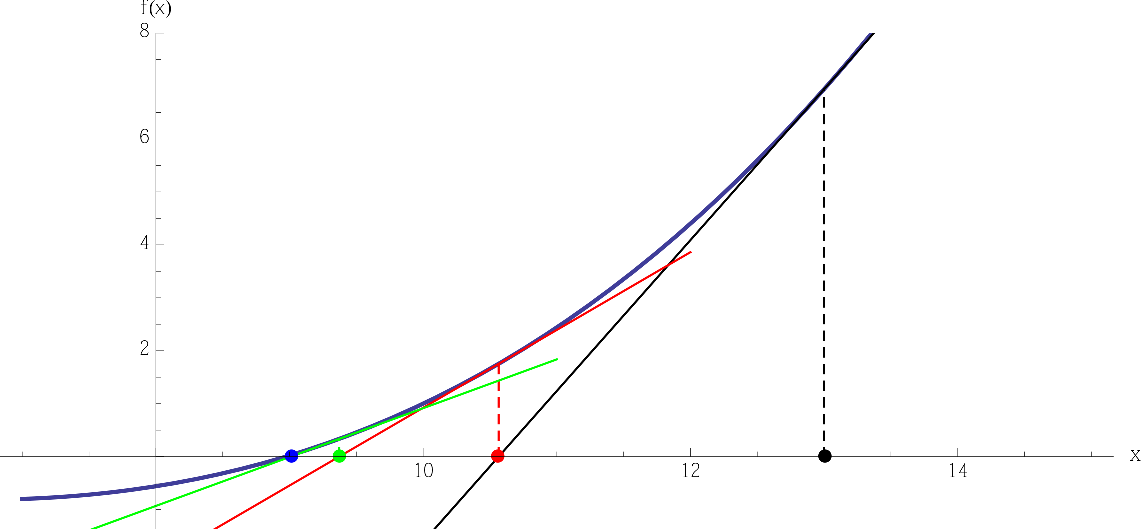
\includegraphics[width=\textwidth]{NRMethod}
\caption{A demonstration of Newton's method in 1D on a simple function with the root at $x_r \approx 8.98$. Starting at $x_0$ = 13, the method converges to within $10^{-4}$ in just three steps.}\label{fig:Newton}
\end{figure}  
\subsection{The Generalized Minimum Residual Method}

There are a vast quantity of residual minimization algorithms in existence, each typically optimized for a particular class of problem. {\tt Channelflow} uses the {\bf G}eneralized {\bf M}inimum {\bf RES}idual (GMRES) method, a Krylov subspace method developed in 1986 by Saad and Schultz\rf{Saad1986}. To illustrate the principle of GMRES, consider the least squares problem of finding the $\Vector{x}$ that minimizes
\begin{equation}\label{eq:AXB}
||\mathbb{A}\Vector{x} -\Vector{b}|| = r.
\end{equation}

\subsubsection{The Krylov Subspace}
Instead of searching for $\Vector{x}$ in the full vector space of the problem, Krylov methods restrict the space to a {\bf Krylov subspace}. The $k$-th Krylov subspace for a matrix $\mathbb{A}$ and a vector $\Vector{c}$, with a guess $\Vector{x}_0$ is defined
\begin{equation}\label{eq:krylov}
\mathcal{K}_k(\mathbb{A},\Vector{c}) = \mathrm{span}\paren{\Vector{c},\mathbb{A}\Vector{c},\mathbb{A}^2\Vector{c}...,\mathbb{A}^{k-1}\Vector{c}}.
 \end{equation}
In practice, $\Vector{c}$ is often set to equal $\Vector{b} - \mathbb{A}\Vector{x}_0$, since it allows for the calculation of convergence estimates.\rf{Ipsen1998}. The motivation for searching for the solution to \refeq{eq:AXB} in the Krylov subspace can be made clear if we consider a slight rearrangement of \refeq{eq:AXB},
 \begin{equation}
 \Vector{x} = \mathbb{A}^{-1}\Vector{b},
 \end{equation}
 from which it is clear that if $\mathbb{A}^{-1}$ can be written as a power series of $\mathbb{A}$, $\Vector{x}$ lies in the Krylov subspace. This can be shown via consideration of the characteristic polynomial of $\mathbb{A}$, and is proved in\rf{Ipsen1998}. 
 
 \subsubsection{The Arnoldi Iteration}
 
Unfortunately, the set of vectors generated by \refeq{eq:krylov} is not guaranteed to form an orthonormal basis, so in practice the Krylov subspace is generated via \refAlg{alg:Arnoldi}, known as the {\bf Arnoldi Iteration}. 
\begin{algorithm}\label{alg:Arnoldi}
Begin with $\Vector{q}_1 = \Vector{b} - \mathbb{A}\Vector{x}_0$. Then for the $k$-th Arnoldi iteration,
\begin{enumerate}
\item calculate $h_{ij} = \mathbb{A}\Vector{q}_{i} \cdot \Vector{q}_j,$ for $i = 1,2,...,j$,
\item generate $\Vector{p} = \mathbb{A}\Vector{q}_j - \sum{i=1}{j}{h_{ij}\Vector{q}_i},$ 
\item and normalize $\Vector{q}_{j+1} = \frac{\Vector{p}}{||p||},$
\end{enumerate}
for $j = 1,2,...,k$.
\end{algorithm}
Incidentally, the Arnoldi iteration is in general used to solve the eigenvalue problem for a matrix\footnote{That is, solving for the eigenvectors $\Vector{q}_k$ and eigenvalues $\lambda_k$ that satisfy $\mathbb{A}\Vector{q}_k = \lambda_k\Vector{q}_k$}, which will prove to be useful later. If we let $\mathbb{Q}_k = [ \Vector{q}_1| \Vector{q}_2 | ... |\Vector{q}_k ]$, and $[\mathbb{H}_k]_{ij} = h_{ij}$ if $h_{ij}$ exist, and $0$ otherwise, then 
\begin{equation}
\mathbb{H}_k = \mathbb{Q}_k^* \mathbb{A}\mathbb{Q},
\end{equation}
and 
\begin{equation}\label{eq:Qiter}
\mathbb{A}\mathbb{Q}_k = \mathbb{Q}_{k+1}\mathbb{\tilde{H}}_k,
\end{equation}
where $\mathbb{\tilde{H}}_k$ is $\mathbb{H}_k$ with an additional row $[0,0,0...,h_{k+1,k}]$. Following the derivation in \rf{Ipsen1998}, if $\Vector{z} \in \mathcal{K}_k(\mathbb{A},\Vector{c})$, 
\begin{equation}
\Vector{z} = \mathbb{Q}_k \Vector{y},
\end{equation}
for some $\Vector{y}$. Then 
\begin{align}
\begin{split}
\mathbb{A}\Vector{z} &= \mathbb{A}\mathbb{Q}_{k}\Vector{y},\\
				&= \mathbb{Q}_{k+1}\mathbb{\tilde{H}}_{k}\Vector{y},
\end{split}
\end{align}
and
\begin{align} 
\begin{split}
\Vector{c} &= ||\Vector{b} - \mathbb{A}\Vector{x}||\Vector{q}_1, \\
	&= ||\Vector{b} - \mathbb{A}\Vector{x}||\Vector{q}_1,\\
	&= ||\Vector{b} - \mathbb{A}\Vector{x}||\mathbb{Q}_{k+1}\Vector{e}_1,
\end{split}
\end{align}
where $\Vector{e}_1$ is the first standard basis vector. This changes the least squares problem from finding the $\Vector{x}$ that minimizes \refeq{eq:AXB} to the $\Vector{y}$ that minimizes
\begin{equation}\label{eq:GMRESMIN}
|| \paren{||\Vector{b} - \mathbb{A}\Vector{x}||}\Vector{e}_1 - \mathbb{\tilde{H}}_k \Vector{y} || = r,
\end{equation}
and is solved by \refAlg{alg:GMRES}.
  \begin{algorithm}\label{alg:GMRES}
   Begin with
 \begin{align*}
 \Vector{c} &= \Vector{b} - \mathbb{A}\Vector{x}_0,\\
  \Vector{q}_1 &= \frac{\Vector{c}}{||c||}, \\
  \mathbb{Q}_1 &= \Vector{q}_1,\\
  \mathcal{K}_1(\mathbb{A},\Vector{c}) &= \mathrm{span}(\Vector{q}_1).
  \end{align*}
  Then the $k$-th GMRES iteration is given by  
  \begin{enumerate}
  \item generating $\Vector{q}_{k+1}$, $\mathbb{Q}_{k+1}$ and $\mathbb{\tilde{H}}_k$ via the Arnoldi iteration,
  \item finding the $\Vector{y}_{k+1}$ that minimizes \refeq{eq:GMRESMIN},
  \item and computing $\Vector{x}_{k+1} = \mathbb{Q}_{k+1}\Vector{y}_{k+1}$.
  \end{enumerate}
  \end{algorithm}

 The second step of \refAlg{alg:GMRES} may seem nonsensical - why have we put this much effort into getting an equation similar to \refeq{eq:AXB}? The key lies in realizing that the minimization problem in  \refAlg{alg:GMRES} has a dimension of $k$, whereas \refeq{eq:AXB} has a dimension on the order of $10^5$. Since the matrix inversion problem scales as dimension to the third power, this reduction is extremely powerful -- especially since GMRES converges quickly -- in this thesis, GMRES rarely took more than 20 iterations to converge. The minimization step in  \refAlg{alg:GMRES} can be solved via a QR decomposition, with a time complexity of $O(n)$\rf{Trefethen1997}.  
 
 \subsection{The Hookstep}
 
 While the Newton method is incredibly powerful, it needs to be provided a sufficiently good guess to stand a chance of converging to a solution. However, in practice, we may be limited in our ability to provide good guesses with our computing resources, and thus need a method of dealing with less than ideal guesses. One major issue with a suboptimal guess is that the linear model used in deriving Newton's method may not be valid for the Newton step $\Vector{dx}_N$, as in \refFig{fig:NewtonOvershoot}. 
  \begin{figure}[h]
 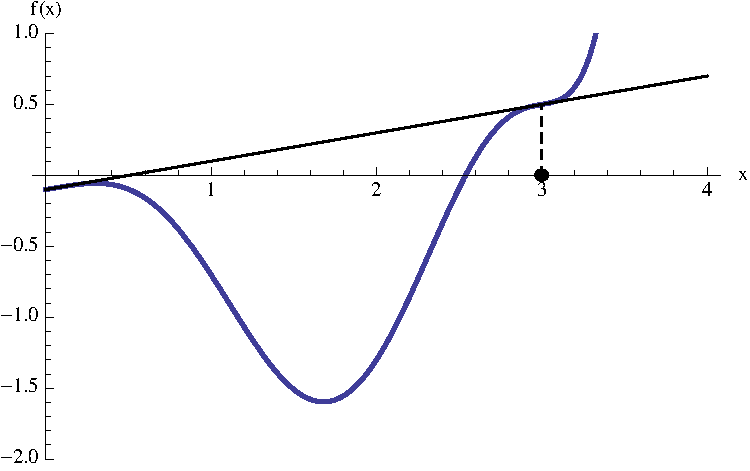
\includegraphics[width=\textwidth]{NewtonOvershoot}
 \caption{If we assume the linear model remains valid for the entire step, we can sometimes be led astray. Because the function becomes rapidly nonlinear, the Newton step takes us very far away from the actual root we are trying to find, and will likely never converge.}\label{fig:NewtonOvershoot}
 \end{figure}
 
 If this is the case, switching to a constrained {\bf hookstep} can force the algorithm to take artificially smaller steps, until the linear model becomes locally accurate. In {\tt Channelflow}, the equation of constraint for the hookstep $\Vector{dx}_H$ is 
 \begin{equation}\label{eq:HSEOC}
 ||\Vector{dx}_H|| \leq \delta,
 \end{equation}
 where $\delta$ is the {\bf trust region} of the linear model, which is recomputed whenever the linear model changes significantly. The hookstep is further restricted to lie in the $k$-th Krylov subspace, so that 
 \begin{equation}\label{eq:HSKRYPROJ}
 \Vector{dx}_H = \mathbb{Q}_{k}\Vector{s},
 \end{equation} 
 where $\Vector{s}$ is now the $k$-dimensional step we need to take. As with the Newton step, the hookstep is determined using GMRES. Unlike the Newton step, the minimization stage of \refAlg{alg:GMRES} is not computed via the QR decomposition\rf{Gibson2014}\rf{Viswanath2007}. Instead, we substitute \eqref{eq:Qiter} and \eqref{eq:HSKRYPROJ} into \eqref{eq:AXB}, giving the residual which we wish to minimize with respect to $\Vector{s}$,
 \begin{equation}\label{eq:HSRes}
 ||\mathbb{Q}^{T}_{k+1}\Vector{b}-\mathbb{\tilde{H}}_k\Vector{s}|| = r.
 \end{equation}
 Applying the singular value decomposition $\mathbb{\tilde{H}}_k = \mathbb{U}\mathbb{D}\mathbb{V}^T$ transforms \eqref{eq:HSRes} intro
 \begin{equation}
 || \Vector{\hat{b}}-\mathbb{D}\Vector{\hat{s}} || = r,
 \end{equation}
 where $\Vector{\hat{s}} = \mathbb{V}^T\Vector{s}$, $\Vector{\hat{b}} = \mathbb{U}^T\mathbb{Q}^T_{k+1}\Vector{b}$, $\mathbb{U},\mathbb{V}$ are square, unitary matricides and $\mathbb{D}$ is a rectangular diagonal matrix. Using Lagrange multipliers, the minimization problems yields the solution\rf{Gibson2014}
 \begin{equation}
 {\hat{s}}_i = \frac{{\hat{b}}_i {D}_{ii}}{{D}_{ii}^2 + \mu},
 \end{equation}
 where $\mu$ minimizes 
 \begin{equation}
 ||\Vector{\hat{s}}(\mu)||^2 - \delta^2 = \mathfrak{r},
 \end{equation}
 which can be trivially solved by a 1D Newton method. 
 
 \section{Recurrence Diagrams}
 
 While the augmentation of the Newton-Krylov method by the hookstep makes it more resilitent against poor guesses, the Newton-Krylov-Hookstep (NKH) method remains extremely sensitive to initial conditions. As a result, an method to generate decent guesses to kickstart the NKH solver is vital. The method used in this thesis is as follows:

 The key here is then to find an intelligent low dimensional projection. One possibility is to view the trajectory in the dissipation and energy input plane, as in\rf{Viswanath2007}, which has proven successful in the past. A better approach, however, is to consider the {\bf recurrence diagram} of the trajectory, which can be generated via \refAlg{alg:rec}. \\
 
  \begin{algorithm}\label{alg:rec}
  \textcolor{white}{haha}
 \begin{enumerate}
 \item Begin with an initial condition. This can be chosen by randomly generating a field, or making a slight random perturbation off a known \ecs.
 \item Integrate this initial condition forward in time using SBDF3 to obtain a trajectory 
 \item Project this trajectory into some low dimensional basis which naturally provides insight into the dynamical structure
 \item Extract some number of good guesses from this projection, and pass them along to the NKH solver.
 \end{enumerate}
 \end{algorithm} 
 The recurrence diagram of a trajectory is a method by which the spatio-temporal separation of successive flow states in a trajectory can be visually and numerically analyzed. The recurrence diagram is a 2D plot of the values of the function 
 \begin{equation}\label{eq:recurrenceEQ}
 \mathfrak{R}(t,T) = ||\Vector{u}(t+T) - \Vector{u}(t)||,
 \end{equation}
 where minima of $\mathfrak{R}$ may indicate the existence of \ecs. Interpretation of a recurrence diagram is not an exact science - for example, a naive search for the minimum of \refFig{fig:recurrenceMinimum}\footnote{I currently don't have MATLAB, Mathematica or Illustrator, so I'll get these figures done as soon as my laptop gets back. Should be by Monday} would yield all the points for which $T=0$. Experience has shown that long, horizontal streaks of minima correspond to the shadowing of a periodic orbit, and tend to be excellent sources of good guesses for the NKH solver. \\
 
 When streamwise or spanwise symmetry is broken, \refeq{eq:recurrenceEQ} must be modified to allow for the possibility of relative solutions, as the problem now changes to finding minima of 
 \begin{equation}\label{eq:4DrecurrenceEQ}
 \mathfrak{R}(t,T,l_x,l_z) = ||\tau(l_x,l_z)\Vector{u}(t+T) - \Vector{u}(t)||.
  \end{equation}
   In principle this is now a 3 or 4 dimensional minimization problem, which would normally preclude the use of a visual approach. This issue is resolved by searching for the $(l_x,l_z)$ that minimizes \refeq{eq:4DrecurrenceEQ} for each $(t,T)$, and only plotting those values of $\mathfrak{R}$. Note that time cost of generating the recurrence diagram goes from $O(n^2)$ to $O(n^4)$ as the spanwise and streamwise symmetries are broken. As a result, analyzing the trajectory of a completely asymmetric trajectory is extremely computationally costly.
 
 \section{Parametric Continuation} 
 
 If we have a solution to \refeq{eq:NRResidual} for some control parameters, such as \ReN\ or the cell size, we may wish to see how these solutions vary with these control parameters. Considering the difficulty of running through the 

 
 
 